\section{Proposed Method}
\label{sec.3}

We propose to use a ConvNet-based deep neural network that is trained to optimize an appropriate ranking loss for the task of predicting relative attribute strength. The network architecture consists of two parts, the \textit{feature learning and extraction} part and the \textit{ranking} part.

The feature learning and extraction part takes a fixed size image, $I_i$, as input and outputs the learned feature representation for that image $\psi_i \in \mathbb{R}^d$.
%Different network architectures have been developed in the literature over the past few years, for extracting and learning features in a deep framework that almost all of them are applicable. 
Over the past few years, different network architectures for computer vision problems have been developed. These deep architectures can be used for extracting and learning features for different applications.
For the current work, outputs of an intermediate layer, like the last layer before the probability layer, from a ConvNet architecture (\eg, AlexNet \cite{Krizhevsky2012ImageNetCW}, VGGNet \cite{verydeep} or GoogLeNet \cite{googlenet}) can be incorporated. %used.
\hl{Please include one or two sentences here to show the network architecture you use here. How many conv layers, how many full connected layers!?}

One of the most widely used models for relative attributes in the literature is RankSVM \cite{Joachims2002}. However,
%here, we want a neural network based ranking procedure that accepts relatively ordered pairs of feature vectors as input during training,
in our case, we seek a neural network-based ranking procedure, to which relatively ordered pairs of feature vectors are are provided during training. This procedure should learn to map each feature vector to an absolute ranking, for testing purpose. Burges \etal~\cite{Burges2005} introduced such a neural network based ranking procedure that exquisitely fits our needs. %with our desired properties. The ranking part of our proposed network architecture is thus similar (reffered to as RankNet).
We adopt a similar strategy and thus, the ranking part of our proposed network architecture is analogous to \cite{Burges2005} (referred to as RankNet).

During training for a minibatch of image pairs and their target orderings, the output of the feature learning and extraction part of the network is fed into the ranking part and a ranking loss is computed. The loss is then back-propagated through the network, which enables us to simultaneously learn the weights of both feature learning and extraction (ConvNet) and ranking (RankNet) parts of the network.  
Further with back-propagation we can calculate the derivative of the estimated ordering with respect to the pixel values.
In this way, we can generate saliency maps for each attribute (see section \ref{sec.4.5}). These saliency maps exhibit interesting properties, as they can be used to localize the regions in the image that are informative about the attribute.

\subsection{RankNet: Learning to Rank Using Gradient Descent}\label{sec3.1}

This section briefly overviews the RankNet %\cite{Burges2005} 
procedure in our context.
Given a set (of size $n$) of pairs of sample feature vectors $\big\{( \psi_{1}^{(k)}, \psi_{2}^{(k)} ) | k \in \{1, \dots, n\} \big\} \in \mathbb{R}^{d \times d}$, and target probabilities $\big\{ t_{12}^{(k)} | k \in \{1, \dots, n\} \big\}$, which indicate the probability of  
sample $\psi_{1}^{(k)}$ being ranked higher than sample $\psi_{2}^{(k)}$. 
We would like to learn a ranking function $f : \mathbb{R}^d \mapsto \mathbb{R}$, such that $f$ specifies the ranking order of a set of features. Here, $f(\psi_i) > f(\psi_j)$ indicates that the %model thinks that 
feature vector $\psi_i$ is ranked higher than $\psi_j$, denoted by $\psi_i \triangleright \psi_j$. The RankNet model \cite{Burges2005} provides an elegant procedure based on neural networks 
to learn the function $f$ from a set of pairs of samples and target probabilities.

Denoting $r_i \equiv f(\psi_i)$, RankNet models the mapping from rank estimates to posterior probabilities $p_{ij} = P(\psi_i \triangleright \psi_j)$ using a logistic function 

\begin{equation}
p_{ij} := \frac{1}{1 + e^{-(r_i - r_j)}}.
\label{eq1}
\end{equation}

The loss for the sample pair of feature vectors $(\psi_i, \psi_j)$ along with target probability $t_{ij}$ is defined as

\begin{equation}
C_{ij} := - t_{ij} \log (p_{ij}) - (1 - t_{ij}) \log (1 - p_{ij}),
\label{eq2}
\end{equation}
which is the binary cross entropy loss.
Figure \ref{fig.2} (left) plots the loss value $C_{ij}$ as a function of $r_i - r_j$ for three values of target probability $t_{ij} \in \{0, 0.5, 1\}$. This function is quite suitable for ranking purposes, as it acts differently compared to regression functions.
Specifically, we are not interested in regression instead of ranking for two reasons: First, we cannot regress the absolute rank of images, since the annotations are only available in pairwise ordering for each attribute, in relative attribute datasets (see section \ref{sec.4.1}). Second, regressing the difference $r_i - r_j$ to $t_{ij}$ is inappropriate. To understand this, let's consider the squared loss

\begin{equation}
R_{ij} = \big[(r_i - r_j) - t_{ij}\big]^2,
\end{equation}
which is typically used for regression, illustrated in Figure \ref{fig.2} (right). We observe that the regression loss forces the difference of rank estimates to be a specific value and disallows over-estimation. Furthermore, its quadratic natures makes it %very
sensitive to noise. This sheds light into why regression objective is the wrong objective to optimize when the goal is ranking.

\begin{figure}
    \centering
    \begin{subfigure}
        \centering
        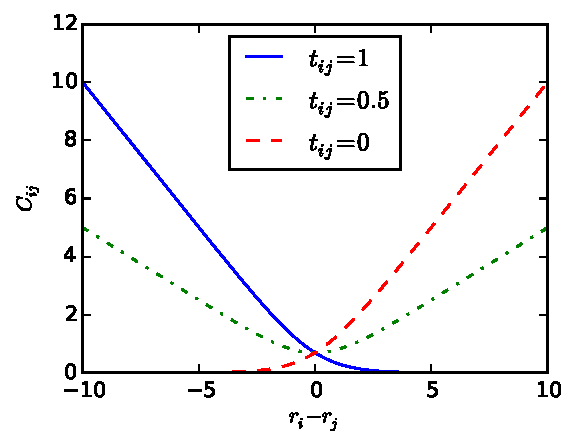
\includegraphics[width=5cm]{fig2-2/fig3.pdf}
    \end{subfigure}
    \begin{subfigure}
        \centering
        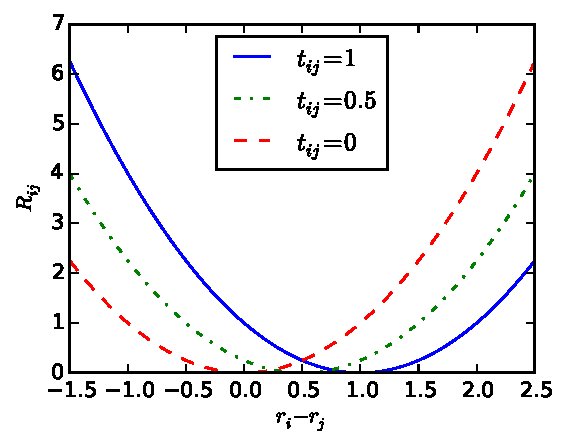
\includegraphics[width=5cm]{fig2-2/fig3-reg.pdf}
    \end{subfigure}
    \caption{The ranking loss value for three values of the target probability (left). The squared loss value for three values of the target probability, typically used for regression (right).}
    \label{fig.2}
\end{figure}

Note that when $t_{ij} = 0.5$, and no information is available about the relative rank of the two samples, the ranking cost becomes symmetric. This can be used as a way to train on patterns that are desired to have similar ranks. This is somewhat not much studied in the previous works on relative attributes.
Furthermore, this model asymptotically converges to a linear function which makes it more appropriate for problems with noisy labels. %than quadratic loss functions.

Training this model is possible using stochastic gradient descent or its variants like RMSProp.
While testing, we only need to estimate the value of $f(\psi_i)$, which resembles the absolute rank of the testing sample. Using $f(\psi_i)$s, we can easily infer both absolute or relative ordering of the testing pairs.


\subsection{Deep Relative Attributes}\label{sec3.2}


Our proposed model is depicted in figure \ref{fig.3}. The model is trained separately, for each attribute. During training, pairs of images $(I_i, I_j)$ are presented to the network, together with the target probability $t_{ij}$. If for the attribute of interest $I_i \triangleright I_j$ (image $i$ exhibits more of the attribute than image $j$), then $t_{ij}$ is expected to be larger than $0.5$ depending on our confidence on the relative ordering of $I_i$ and $I_j$. Similarly, if $I_i \triangleleft I_j$, then $t_{ij}$ is expected to be smaller than $0.5$, and if it is desired that the two images have the same rank, $t_{ij}$ is expected to be $0.5$. Because of the nature of the datasets, we chose $t_{ij}$ from the set $\{0, 0.5, 1 \}$, according to the available annotations in the dataset.


%%%%%%%%%%%%%%%%%%%%%%%% Figure 3 %%%%%%%%%%%%%%%%%%%%%%%%%%%%%%%%%%%%%%%%%%%%%%%%%%%%%
\begin{figure}{t!}
\centering
\resizebox{\linewidth}{!}
{
% We need layers to draw the block diagram
\pgfdeclarelayer{background}
\pgfdeclarelayer{foreground}
\pgfsetlayers{background,main,foreground}

% Define a few styles and constants
\tikzstyle{sensor}=[draw, fill=blue!20, text width=5em, 
    text centered, minimum height=2.5em]
\tikzstyle{ann} = [above, text width=5em]
\tikzstyle{naveqs} = [sensor, text width=6em, fill=red!20, 
    minimum height=12em, rounded corners]
\def\blockdist{2.3}
\def\edgedist{2.5}

\begin{tikzpicture}
    % feature extraction part rectangle
	% images
	\node (im1) at (0cm,1cm) [draw] {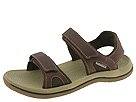
\includegraphics[scale=1]{Fig2/im1.jpg}};
	\node (im2) at (0cm, -6cm) [draw] {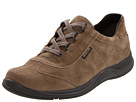
\includegraphics[scale=1]{Fig2/im2.jpg}};

	% topconv1 layer
	\node (tconv1) at (5.1cm, 1cm) {};
%	\draw [fill=blue!20] (5.6cm,3.1cm) rectangle (9.6cm,0.1cm);
	\draw [fill=blue!20] (5.4cm,2.9cm) rectangle (9.4cm,-0.1cm);
	\draw [fill=blue!20] (5.2cm,2.7cm) rectangle (9.2cm,-0.3cm);
	\draw [fill=blue!20] (5cm,2.5cm) rectangle (9cm,-0.5cm);

	% bottomconv1 layer
	\node (bconv1) at (5.1cm, -6cm) {};
%	\draw [fill=blue!20] (5.6cm,-3.9cm) rectangle (9.6cm,-6.9cm);
	\draw [fill=blue!20] (5.4cm,-4.1cm) rectangle (9.4cm,-7.1cm);
	\draw [fill=blue!20] (5.2cm,-4.3cm) rectangle (9.2cm,-7.3cm);
	\draw [fill=blue!20] (5cm,-4.5cm) rectangle (9cm,-7.5cm);

	% arrows from images to conv1s
	\path [draw, ->, line width=3] (im1.east) -- node [above, scale=3] {$I_i$} (tconv1);
	\path [draw, ->, line width=3] (im2.east) -- node [above, scale=3] {$I_j$} (bconv1);

	% topconv2 layer
	\node (tconv2) at (12cm, 1cm) {};
	\draw [fill=blue!20] (12.6cm,3.1cm) rectangle (16.6cm,0.1cm);
	\draw [fill=blue!20] (12.4cm,2.9cm) rectangle (16.4cm,-0.1cm);
	\draw [fill=blue!20] (12.2cm,2.7cm) rectangle (16.2cm,-0.3cm);
	\draw [fill=blue!20] (12cm,2.5cm) rectangle (16cm,-0.5cm);

	% bottomconv2 layer
	\node (bconv2) at (12cm, -6cm) {};
	\draw [fill=blue!20] (12.6cm,-3.9cm) rectangle (16.6cm,-6.9cm);
	\draw [fill=blue!20] (12.4cm,-4.1cm) rectangle (16.4cm,-7.1cm);
	\draw [fill=blue!20] (12.2cm,-4.3cm) rectangle (16.2cm,-7.3cm);
	\draw [fill=blue!20] (12cm,-4.5cm) rectangle (16cm,-7.5cm);

	\path (tconv1.east)+(4.65cm, 0cm) -- node [scale=4]{\dots} (tconv2);
	\path (bconv1.east)+(4.65cm, 0cm) --node [scale=4]{\dots} (bconv2);

	\node (convnet) [below, scale=3.5] at (11cm, -8cm) {ConvNet};

	% toprank
	\node (tconvout) at (16.6cm, 1cm) {};
	\node (trank) at (21.1cm, 1cm) [rectangle, draw, fill=red!20, scale=3, align=center] {Ranking \\  Layer};
	\path [draw, line width=3, ->] (tconvout) -- node[above, scale=3] {$\psi_i$} (trank.west);

	% bottomrank
	\node (bconvout) at (16.6cm, -6cm) {};
	\node (brank) at (21.1cm, -6cm) [rectangle, draw, fill=red!20, scale=3, align=center] {Ranking \\  Layer};
	\path [draw, line width=3, ->] (bconvout) -- node[above, scale=3] {$\psi_j$} (brank.west);

	% shared rank layer
	\node (dashcenter) at (10.75cm, 0cm) {};
	\path [draw, line width=2, <->] (trank.south) -- node [scale=2, draw, rectangle, fill=white, line width=0] {\rotatebox{90}{shared}} (brank.north);
	\path [draw, line width=2, <->] (trank.south -| dashcenter) -- node [scale=2, draw, rectangle, fill=white, line width=0] {\rotatebox{90}{shared}} (brank.north -| dashcenter);

	% posterior
	\node (posterior) at (27cm, -2.5cm) [rectangle, draw, fill=orange!10, scale=3, minimum width=15] {\rotatebox{90}{Posterior}};

	% connect rank layer to posterior
	\path [draw, line width=2, ->] (trank.east) -- node [scale=3, above] {$r_i$} (posterior);
	\path [draw, line width=2, ->] (brank.east) -- node [scale=3, above] {$r_j$} (posterior);

	% BXE
	\node (bxent) at (36cm, -2.5cm) [draw,fill=green!10, regular polygon, regular polygon sides=3, shape border rotate=-90, scale=8, line width=2] {};
	\node at (36.2cm, -2.5cm) {\Huge BXEnt};

	% target value
	\node [draw, rectangle] (target) at (30cm , -4.2cm) [scale=3] {target};

	% connect to bxe
	\draw [line width=3, ->] (posterior.east) -- ++(3cm, 0cm) |- node [above right, scale=3] {$p_{ij}$}  (bxent.north west);
	\draw [line width=3, ->] (target.east) -- node [below, scale=3] {$t_{ij}$}  (bxent.south west |- target.east);

	% loss node
	\node (loss) [scale=3] at (44cm, -2.5cm) { loss};

	% connect bxent to loss
	\draw [line width=3, ->] (bxent.east) -- node [above, scale=3] {$C_{ij}$}  (loss.west);
\end{tikzpicture}}
\caption{The overall schematic view of the proposed method during training. The network consists of two parts, the \textit{feature learning and extraction} part (labeled ConvNet in the figure), and the \textit{ranking} part (the Ranking Layer). Pairs of images are presented to the network with their corresponding target probabilities. This is used to calculate the loss, which is then back-propagated through the network to update the weights.}
\label{fig.3}
\end{figure}
%%%%%%%%%%%%%%%%%%%%%%%% Figure 3 %%%%%%%%%%%%%%%%%%%%%%%%%%%%%%%%%%%%%%%%%%%%%%%%%%%%%



The pair of images then go though the feature learning and extraction part of the network (ConvNet). This procedure maps the images %into
onto feature vectors $\psi_i$ and $\psi_j$, respectively. Afterwards, these feature vectors go through the ranking layer, as described in section \ref{sec3.1}. We choose the ranking layer to be a fully connected neural network layer with linear activation function, a single output neuron and weights $w$ and $b$. It maps the feature vector $\psi_i$ to the estimated absolute rank of that feature vector, $r_i \in \mathbb{R}$, where

\begin{equation}
r_i := w^T \psi_i + b.
\end{equation}

The two estimated ranks $r_i$ and $r_j$, for the two images $I_i$ and $I_j$ in comparison, are then combined (using Equation \eqref{eq1}) to output the estimated posterior probability $p_{ij} = P(I_i \triangleright I_j)$. %and 
This estimated posterior probability is used along with the target probability $t_{ij}$ to calculate the loss, as in Equation \eqref{eq2}. This loss is then back-propagated through the network and is used to update the weights of the whole network, including both the weights of the feature learning and extraction sub-network and the ranking layer.

During testing (Figure \ref{fig.4}), we need to calculate the estimated absolute rank $r_k$ for each testing image $I_k$. Using these estimated absolute ranks, we can then easily infer both the relative or absolute attribute ordering, for all testing pairs.


%%%%%%%%%%%%%%%%%%%%%%%% Figure 4 %%%%%%%%%%%%%%%%%%%%%%%%%%%%%%%%%%%%%%%%%%%%%%%%%%%%%
\begin{figure}
\centering
\resizebox{\linewidth}{!}
{
% We need layers to draw the block diagram
\pgfdeclarelayer{background}
\pgfdeclarelayer{foreground}
\pgfsetlayers{background,main,foreground}

% Define a few styles and constants
\tikzstyle{sensor}=[draw, fill=blue!20, text width=5em, 
    text centered, minimum height=2.5em]
\tikzstyle{ann} = [above, text width=5em]
\tikzstyle{naveqs} = [sensor, text width=6em, fill=red!20, 
    minimum height=12em, rounded corners]
\def\blockdist{2.3}
\def\edgedist{2.5}

\begin{tikzpicture}
	\node (im1) at (0cm,1cm) [draw] {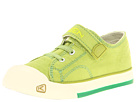
\includegraphics[scale=1]{Fig1/pair3A.jpg}};

	% topconv1 layer
	\node (tconv1) at (5.1cm, 1cm) {};
	\draw [fill=blue!20] (5.4cm,2.9cm) rectangle (9.4cm,-0.1cm);
	\draw [fill=blue!20] (5.2cm,2.7cm) rectangle (9.2cm,-0.3cm);
	\draw [fill=blue!20] (5cm,2.5cm) rectangle (9cm,-0.5cm);

	% arrows from images to conv1s
	\path [draw, ->, line width=3] (im1.east) -- node [above, scale=3] {$I_k$} (tconv1);

	% topconv2 layer
	\node (tconv2) at (12cm, 1cm) {};
	\draw [fill=blue!20] (12.6cm,3.1cm) rectangle (16.6cm,0.1cm);
	\draw [fill=blue!20] (12.4cm,2.9cm) rectangle (16.4cm,-0.1cm);
	\draw [fill=blue!20] (12.2cm,2.7cm) rectangle (16.2cm,-0.3cm);
	\draw [fill=blue!20] (12cm,2.5cm) rectangle (16cm,-0.5cm);

	\path (tconv1.east)+(4.65cm, 0cm) -- node [scale=4]{\dots} (tconv2);

	% toprank
	\node (tconvout) at (16.6cm, 1cm) {};
	
	\node (trank) at (21.5cm, 1cm) [rectangle, draw, fill=red!20, scale=3, align=center] {Ranking \\  Layer};
	\path [draw, line width=3, ->] (tconvout) -- node[above, scale=3] {$\psi_k$} (trank.west);
	
	% posterior
	\node (posterior) at (26.5cm, 1cm){};

	% connect rank layer to posterior
	\path [draw, line width=3, ->] (trank.east) -- node [scale=3, above] {$r_k$} (posterior);

	
\end{tikzpicture}}
\caption{During testing, we only need to evaluate $r_k$ for each testing image. Using this value, we can infer the relative or absolute ordering of testing images, for the attribute of interest.}
\label{fig.4}
\end{figure}
%%%%%%%%%%%%%%%%%%%%%%%% Figure 4 %%%%%%%%%%%%%%%%%%%%%%%%%%%%%%%%%%%%%%%%%%%%%%%%%%%%%